%%%%%%%%%%%%%%%%%%%%%%%%%%%%%%%%%%%%%%%%%%%%%%%%%%%%%%%%%%%%%%%%%
% Dissertacao de Mestrado / Dept Fisica, CFM, UFSC              %
% Lacerda@UFSC - 2013                                           %
%%%%%%%%%%%%%%%%%%%%%%%%%%%%%%%%%%%%%%%%%%%%%%%%%%%%%%%%%%%%%%%%%


%:::::::::::::::::::::::::::::::::::::::::::::::::::::::::::::::%
%                                                               %
%                          Capítulo 4                           %
%                                                               %
%:::::::::::::::::::::::::::::::::::::::::::::::::::::::::::::::%

%***************************************************************%
%                                                               %
%                       Testes com PCA                          %
%                                                               %
%***************************************************************%

\chapter{PCA nos espectros}
\label{sec:UsoPCA}

O uso de métodos estatísticos já se estende por séculos em praticamente todas (senão todas) as áreas de conhecimento.
Esse fato cria uma necessidade de que existam cada vez mais estudos sobre estudos, ou {\em metaestudos}\footnote{Em
alusão a metadados, que são dados sobre dados.}. Precisamos saber de que maneira os pré-processamentos de nossa amostra
afetam os dados e, principalmente, o resultado após a aplicação de determinada técnica, para que dessa forma o
desenvolvimento não se torne uma ``caixa preta'' inacessível.

\section{Pré-processamento dos cubos}
\label{sec:UsoPCA:PCAlidades}

Antes dos espectros chegarem ao PyCASSO, todas as informações de {\em flags}\footnote{Marcações.} em {\em bad pixels} e
linhas telúricas\footnote{Linhas de absorção referentes à atmosfera.} são criadas em um pipeline de pré-processamento
chamado {\sc qbick}. Esse pipeline também prepara os cubos para a execução do \starlight, e para organização deles pelo
PyCASSO, definindo as zonas de Voronoi, a reamostragem em $\lambda$ e colocando os espectros em repouso usando o {\em
redshift} calculado dentro dos $5"$ centrais da galáxia. Todas essas informações e pré-processamentos provenientes de
{\sc qbick} são herdadas pelo PyCASSO e já estão contidadas em seus cubos de espectros.

Apesar desses pré-processamentos supracitados, não é sobre eles vamos falar aqui, e sim sobre aqueles que são feitos nos
espectros contidos no PyCASSO antes da aplicação do PCA. Como o PCA é uma técnica em qual calcula-se os eixos que,
através da variância, melhor expandem sua base de dados, é natural que qualquer pré-processamento que altere a variância
dos dados, resultará num conjunto diferente de PCs. Quando aplicamos o PCA aos cubos do CALIFA estamos buscando
variâncias espaciais nos espectros. Durante nossas investigações fizemos uma série de testes com pré-processamentos nos
espectros. Dois deles são constantes em todos os estudos (Figura \ref{fig:UsoPCA:checkmask}). Primeiro todos os
espectros são limitados ao intervalo de $3800$ a $6850$ \AA. Após essa limitação, são removidas todas as linhas
telúricas. Fazemos então uma estatística com todos os {\em bad pixels} de cada cubo, assim, todos aqueles que estão
presentes em $90\%$ dos espectros são removídos. Cabe aqui lembrar que todos os espectros precisam ter os mesmos pontos
em $\lambda$ pois precisamos construir a matriz de covariância. \fixme\textcolor{red}{ARRUMAR CÓDIGO PCALIFA E GERAR
GRÁFICOS OU TABELA}

\begin{figure}
    %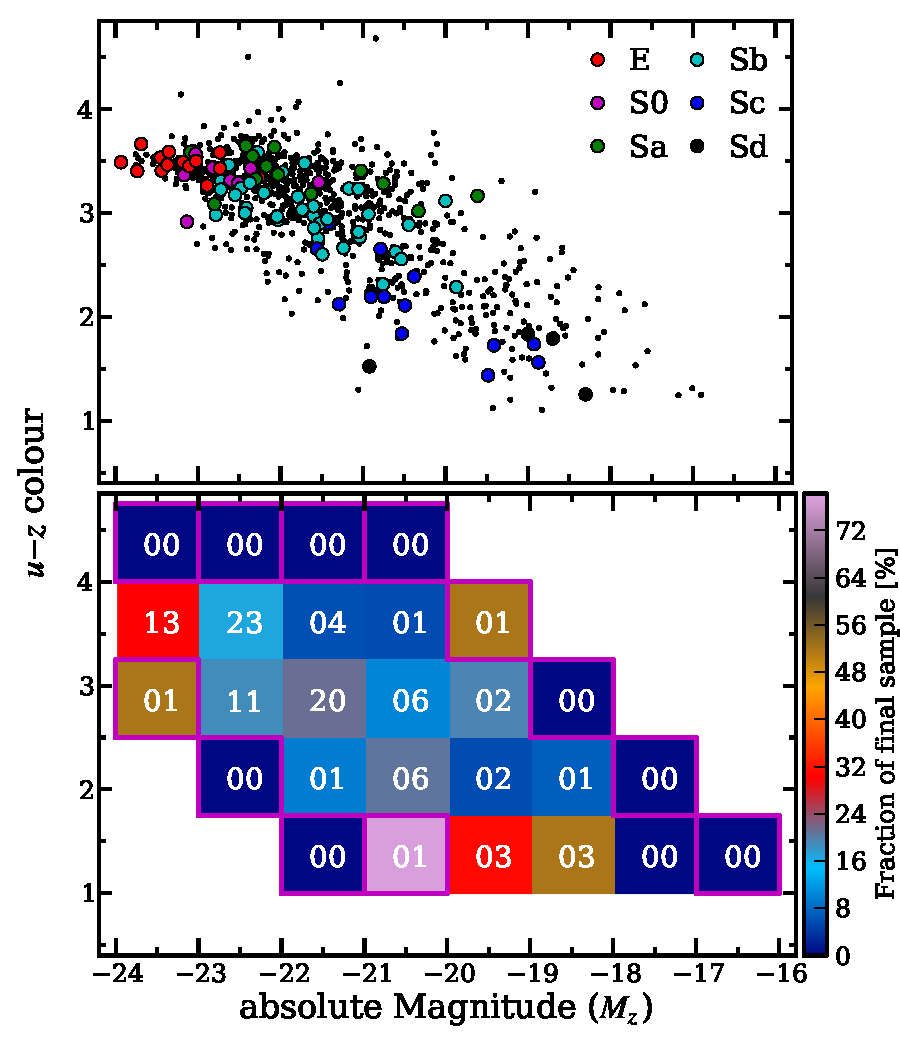
\includegraphics[height=0.5\textwidth]{figuras/figHusemann2013Fig2.pdf}
    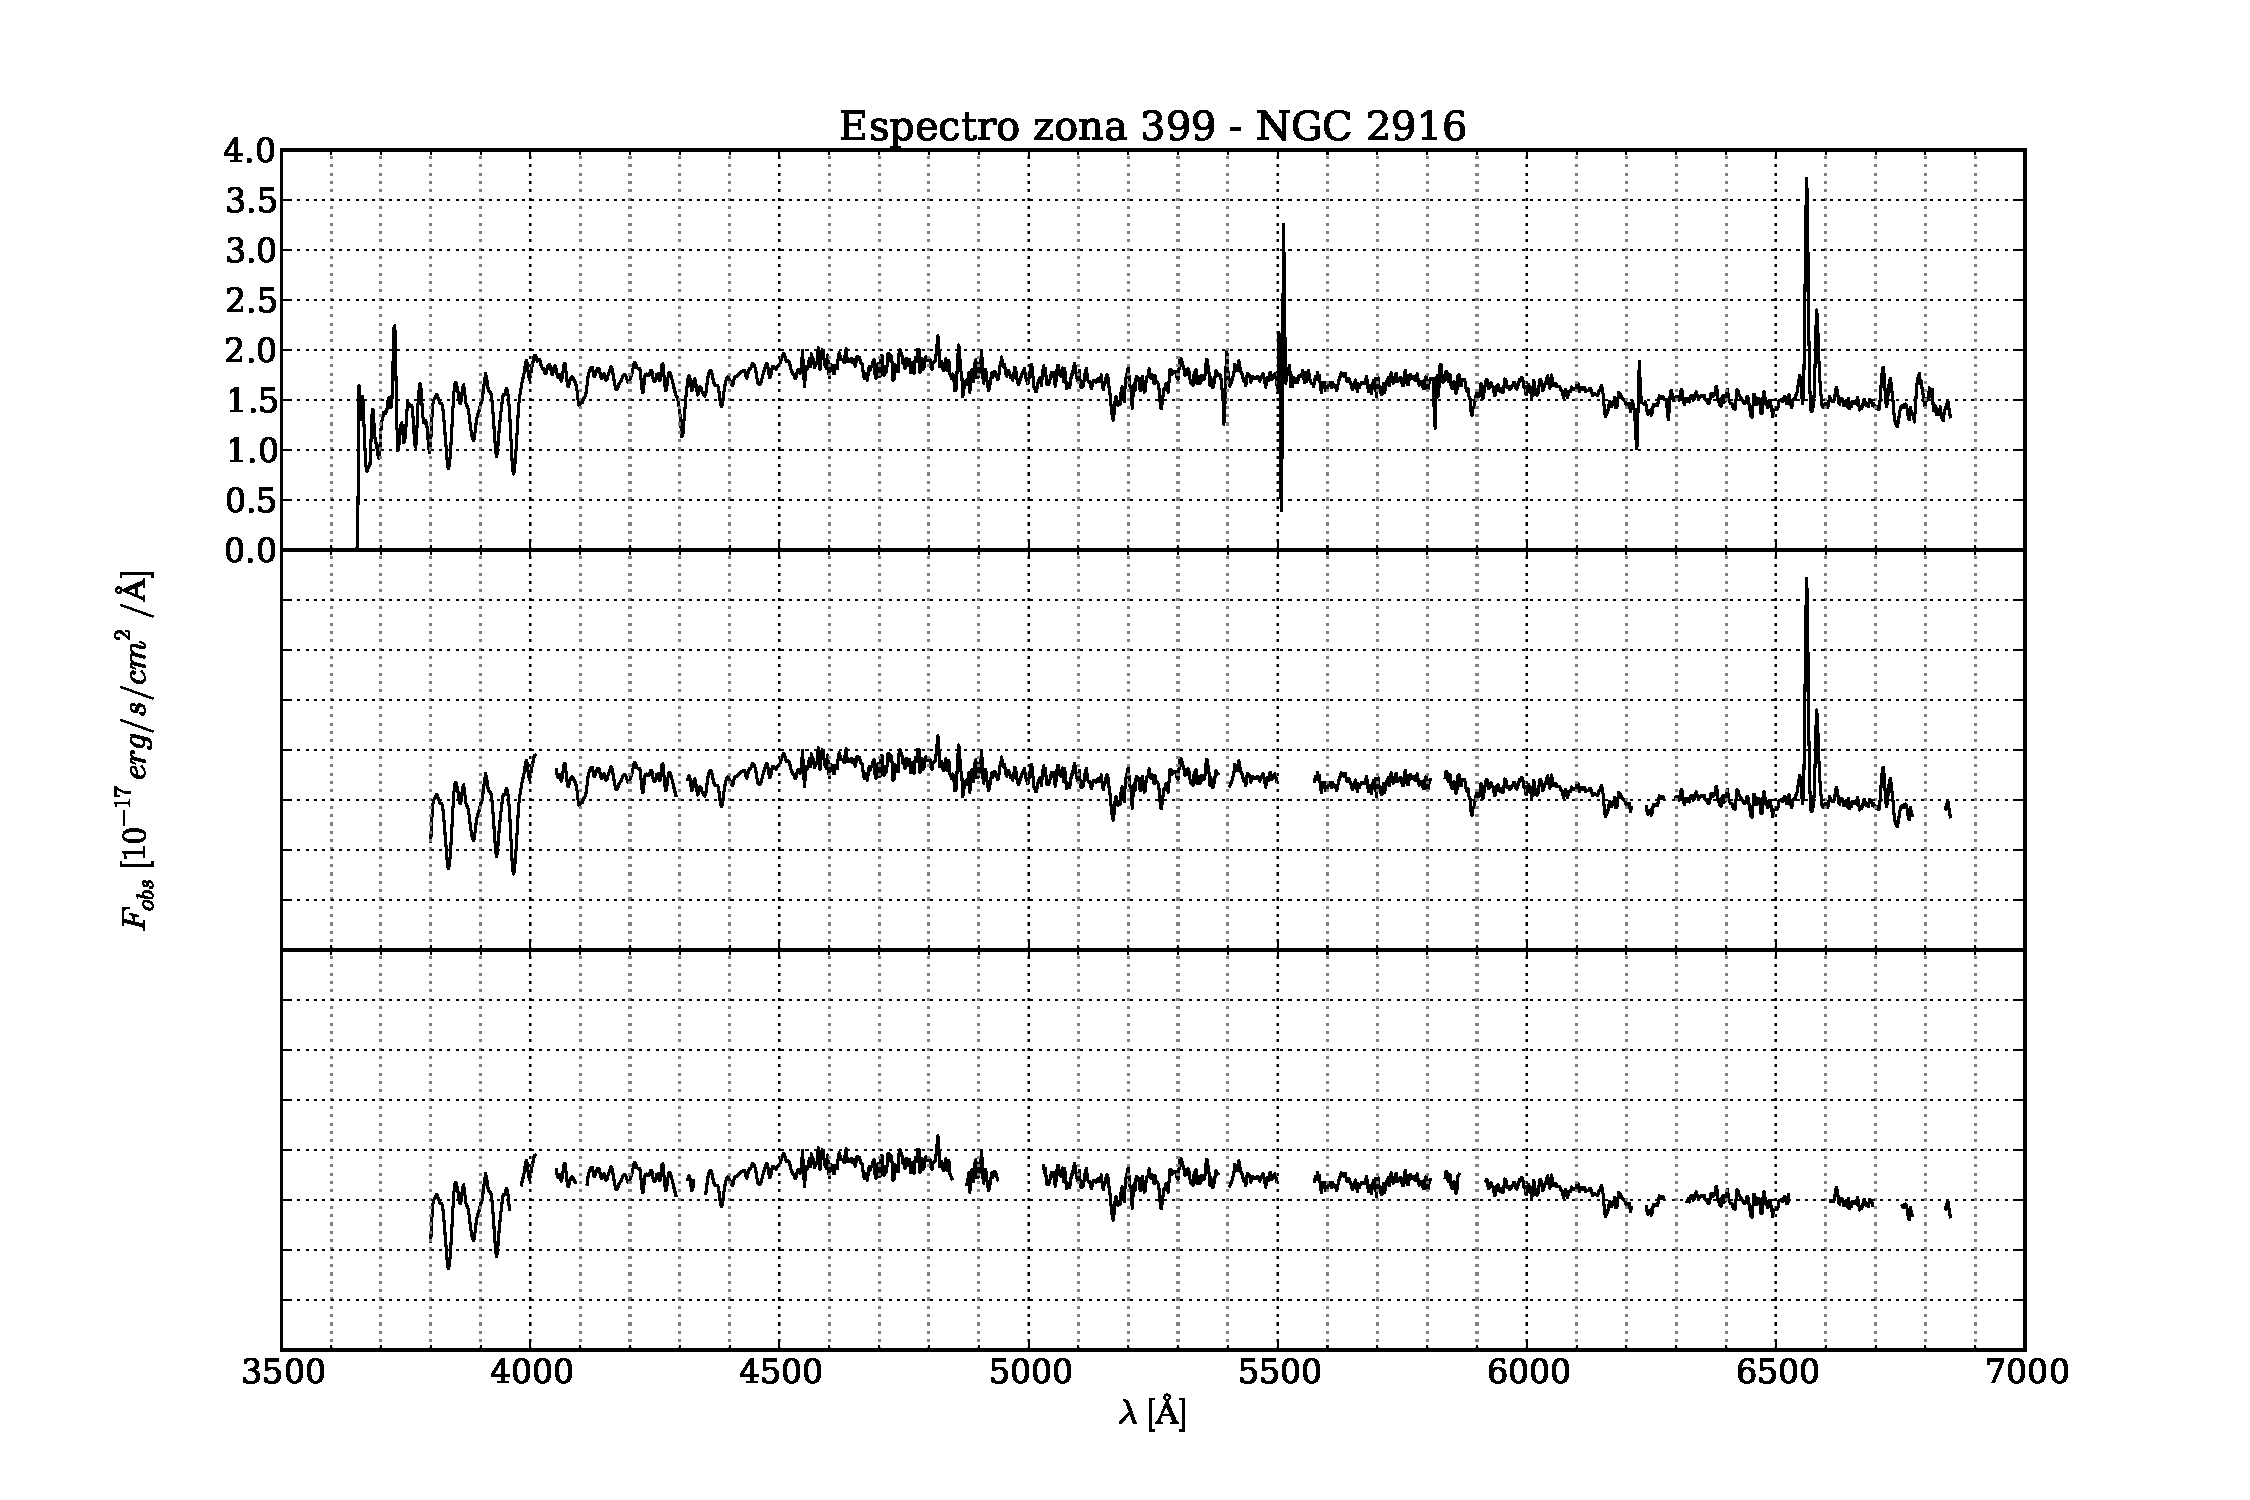
\includegraphics[width=1.0\textwidth]{figuras/K0277-constant_inital_mask-399.pdf}
    \caption[Exemplo de máscaras em um espectro do cubo de dados.]
    {Espectro da zona 399 da galáxia NGC 2916 (CALIFA 277). Acima está o espectro completo. No segundo vemos o espectro
    com linhas telúricas e bad-pixels removidos, além do limite de intervalo em comprimendo de onda de $3800$ a $6850$
    \AA. No espectro mais abaixo, além das partes removidas no segundo, estão foram removidas também as mesmas linhas de
    emissão mascaradas na síntese de populações estelares.}
    \label{fig:UsoPCA:checkmask}
\end{figure}

\subsection{Normalização}
\label{sec:UsoPCA:PCAlidades:norm}

Após esses dois pré-processamentos constantes em todos os cubos podemos fazer uma normalização nos espectros. No caso do
CALIFA, o cubo de espectros inclui um {\em FoV} que abrange praticamente toda a galáxia. Isso gera uma variância
indevida entres as zonas devido a luminosidade mais intensa nas zonas centrais da galáxia em comparação com as mais
afastadas. Indevidas pois não trazem informação nova para a nossa análise. Cada espectro é então normalizado pelo seu
fluxo em $5635$ \AA. Podemos ver um exemplo da diferença nas PCs na figura \fixme \textcolor{red}{GERAR GRÁFICOS}.

\subsection{Fluxos observados e sintéticos}
\label{sec:UsoPCA:PCAlidades:flux}

\fixme \textcolor{red}{Isso não é um pré-processamento\ldots aonde colocar???}

Com o PyCASSO, temos o resultado da síntese de populações estelares já organizado para as galáxias do CALIFA. Com isso
realizamos o PCA no cubo de espectros observados e no de espectros sintéticos, com e sem normalização. A grande
diferença é que nos espectros sintéticos estão contidas apenas as informações sobre populações
estelares\footnote{Suavização, correções por poeira e cinemática também são feitas nos espectros no processo de síntese.
Mais detalhes em \citet{CidFernandes2005}}.

\subsection{Linhas de emissão e intervalos específicos em comprimento de onda}
\label{sec:UsoPCA:PCAlidades:emlin}

Nos espectros, além dos {\em bad pixels} e linhas telúricas, podemos mascarar regiões desnecessárias para determinada
investigação científica. Nosso foco é o estudo das populações estelares, portanto necessitamos que as linhas de emissão,
geralmente associadas ao gás presente nas galáxias \fixme sejam removidas do espectro. Dessa forma podemos fazer
correlações entre os resultados do PCA e as propriedades físicas obtidas pela síntese.

Podemos também executar o PCA apenas em intervalos específicos do espectro. Isso pode ser feito de várias formas, por
exemplo utilizando todos os pontos do(s) intervalo(s) em $\lambda$, ou utilizando apenas o fluxo integrado, ou apenas
larguras equivalentes de linhas, ou FWHM das linhas. Um exemplo aplicado é fazer o PCA apenas das regiões que abrangem
$\oIII/\Hbeta$ em conjunto com $\nII/\Halpha$ ou então $\mathrm{H}\delta$ e D$4000$ para estudar a variância espacil
desses ratios.

Nas nossas análises no próximo capítulo \ref{sec:result} são mascaradas também todas as regiões que são removidas na
síntese ($\mathrm{H}\epsilon$: de $3960$ a $3980$ \AA; $\mathrm{H}\delta$: de $4092$ a $4112$ \AA; $\mathrm{H}\gamma$:
de $4330$ a $4350$ \AA; \Hbeta: de $4848$ a $4874$ \AA; \oIII: de $4940$ a $5028$ \AA; $\mathrm{He\,\textsc{i}}$ e
$\mathrm{NaD}$: de $5866$ a $5916$ \AA; \Halpha e \nII: de $6528$ a $6608$ \AA; $\mathrm{S\,\textsc{ii}}$: de $6696$ a
$6752$ \AA).

\subsection{Cinemática}
\label{sec:UsoPCA:PCAlidades:cinem}

Pelo amplo {\em FoV} que as observações do CALIFA são feitas é normal que existam espectros que estão deslocados para o
azul ({\em blue-shifted}) ou para o vermelho ({\em red-shifted}) dependendo da velocidade de rotação projetada. A
disperção de velocidades em cada ponto da galáxia também pode causar alargamento ou estreitamento das linhas. Ambos
efeitos cinemáticos (velocidade e dispersão de velocidades) também causam um grande disperdício de variâncias. É normal
que ambos sempre apareçam entre as primeiras PCs, como será visto no capítulo posterior. Esse tipo de informação não nos
interessa pois não adiciona informações, a priori, sobre as populações estelares, além de existirem métodos mais
eficazes e direcionados para a determinação de propriedades cinemáticas.

\ldots \dots \ldots \ldots

\textcolor{red}{DAQUI PRA BAIXO AINDA É O ESQUELETO}
\ojo A Filosofia desse capítulo é aprender/testar como operar o PCA para que ele
reflita isso ou aquilo... descrevemos uma série de experimentos nesse sentido.

Preprocessamentos e diferentes tipos de PCAs com ou sem linhas, diferentes
faixas espectrais, com dados normalizados ou não. (importante!!!)

Vamos nos limitar a no-emission lines analysis, descrever a máscara de linhas de
emissão, etc. Isso para facilitar a coisa e pq queremos correlar o resultado do
PCA com os dados do Starlight (PyCASSO).

Simulações para ajudar a decifrar os resultador, população jovem + velha +
modelo de distribuição espacial - ver efeitos de estratégias de
preprocessamento.

Correlacionando os resultados do PCA com as propriedades do starlight (tipo de
engenharia reversa)

Linhas telúricas - remover ou não... bad pixels... mascarar ou não linhas de
emissão